\documentclass[12pt]{article}
%%%%%%%%%%%%%%%%%%%%%%%%%%%%%%%%%%%%%%%%%%%%%%%%%%%%%%%%%%%%%
%% Document setup for Syllabus and HW

\textwidth=7in
\textheight=9.5in
\topmargin=-1in
\headheight=0in
\headsep=.5in
\hoffset  -.85in

\usepackage{amsmath} % for \text{}
\usepackage{amsfonts} % For \text{}
\usepackage{amssymb} % For \text{}
\usepackage{nth}
\usepackage{enumerate}
%\usepackage{nth}

%% Stolen from Nathan Baker
\newcommand{\erf}{{\mathrm{erf}}}
\newcommand{\erfc}{{\mathrm{erfc}}}
\newcommand{\erfi}{{\mathrm{erfi}}}
\newcommand{\argh}{{\mathrm{arg}}}
\newcommand{\atan}{{\mathrm{atan}}}
\newcommand{\acos}{{\mathrm{acos}}}
\newcommand{\asin}{{\mathrm{asin}}}
\newcommand{\mat}[1]{\,\underline{\underline{#1}}\,}
\newcommand{\abs}[1]{\left| #1 \right|}
\newcommand{\norm}[1]{\left\| #1 \right\|}
\newcommand{\order}[1]{{\mathcal{O}} \left( #1 \right)}
\newcommand{\op}[1]{{\mathcal{#1}}}
\newcommand{\myfile}[1]{\texttt{#1}}
\newcommand{\myvar}[1]{\textsf{#1}}
\newcommand{\mean}[1]{{\left\langle {#1} \right\rangle}}

% The master boolean -- set this to "masterfalse" or "mastertrue"
%\newif\ifmaster \masterfalse
\newif\ifmaster \masterfalse
\newif\ifmaster \mastertrue

%http://tex.stackexchange.com/questions/145812/using-fbox-in-a-newenvironment
\newcommand\notes[1]{%
  \fbox{\begin{minipage}{0.9\textwidth}#1\end{minipage}}}

%%\newcommand{\hidesolution}[1]{ \ifmaster { {#1} } \else { {Go to class.} } \fi }
%%\newcommand{\hideanswer}[1]{ \ifmaster { #1 } \else {} \fi }
%%\newcommand{\solution}[1]{ \begin{proof}[Solution] \hidesolution{#1} \end{proof} }
%%\newcommand{\answer}[1]{ \hideanswer{\newpage\ \newpage \notes{\begin{proof}[Answer] #1 \end{proof}}} }

%% MGL
\newcommand{\CC}{\mathbb{C}}
\newcommand{\N}{\mathbb{N}}
%\newcommand{\vect}[1]{\,\vec{\mathbf{#1}}\,}
\newcommand{\vect}[1]{\,\mathbf{#1}\,}
\usepackage{tabularx}
\newcommand{\vtau}{\vect{\tau}}
\newcommand{\va}{\vect{a}}
\newcommand{\vb}{\vect{b}}
\newcommand{\vc}{\vect{c}}
\newcommand{\vd}{\vect{d}}
\newcommand{\ve}{\vect{e}}
\newcommand{\vf}{\vect{f}}
\newcommand{\vg}{\vect{g}}
\newcommand{\vh}{\vect{h}}
\newcommand{\vi}{\vect{i}}
\newcommand{\vj}{\vect{j}}
\newcommand{\vk}{\vect{k}}
\newcommand{\vl}{\vect{l}}
\newcommand{\vm}{\vect{m}}
\newcommand{\vn}{\vect{n}}
\newcommand{\vo}{\vect{o}}
\newcommand{\vp}{\vect{p}}
\newcommand{\vq}{\vect{q}}
\newcommand{\vr}{\vect{r}}
\newcommand{\vs}{\vect{s}}
\newcommand{\vt}{\vect{t}}
\newcommand{\vu}{\vect{u}}
\newcommand{\vv}{\vect{v}}
\newcommand{\vw}{\vect{w}}
\newcommand{\vx}{\vect{x}}
\newcommand{\vy}{\vect{y}}
\newcommand{\vz}{\vect{z}}

\newcommand{\vA}{\vect{A}}
\newcommand{\vB}{\vect{B}}
\newcommand{\vC}{\vect{C}}
\newcommand{\vD}{\vect{D}}
\newcommand{\vE}{\vect{E}}
\newcommand{\vF}{\vect{F}}
\newcommand{\vG}{\vect{G}}
\newcommand{\vH}{\vect{H}}
\newcommand{\vI}{\vect{I}}
\newcommand{\vJ}{\vect{J}}
\newcommand{\vK}{\vect{K}}
\newcommand{\vL}{\vect{L}}
\newcommand{\vM}{\vect{M}}
\newcommand{\vN}{\vect{N}}
\newcommand{\vO}{\vect{O}}
\newcommand{\vP}{\vect{P}}
\newcommand{\vQ}{\vect{Q}}
\newcommand{\vR}{\vect{R}}
\newcommand{\vS}{\vect{S}}
\newcommand{\vT}{\vect{T}}
\newcommand{\vU}{\vect{U}}
\newcommand{\vV}{\vect{V}}
\newcommand{\vW}{\vect{W}}
\newcommand{\vX}{\vect{X}}
\newcommand{\vY}{\vect{Y}}
\newcommand{\vZ}{\vect{Z}}
\newcommand{\diffd}{\mathrm{d}}
\newcommand{\deriv}[2]{\frac{\diffd #1}{\diffd #2}} % derivative
%\newcommand{\pd}[2]{\frac{\partial#1}{\partial#2}}
%\newcommand{\dd}[2]{\frac{d#1}{d#2}}
\newcommand{\dinline}[2]{\diffd #1/\diffd #2} % for derivatives
\newcommand{\pdinline}[2]{\partial#1/\partial#2}

%\newcommand{\bra}[1]{\left\langle #1 \right|}
%\newcommand{\ket}[1]{\left| #1 \right\rangle}

\newcommand{\xd}{\dot{x}}

\newcommand{\boldcent}[1] {\begin{center}\textbf{ #1 }\end{center}}
% ***********************************************************
% ******************* PHYSICS HEADER ************************
% ***********************************************************
% From http://www.dfcd.net/articles/latex/latex.html
% Version 2
%\documentclass[11pt]{article} 
\usepackage{amsmath} % AMS Math Package
\usepackage{amsthm} % Theorem Formatting
\usepackage{amssymb}	% Math symbols such as \mathbb
\usepackage{graphicx} % Allows for eps images
\usepackage{multicol} % Allows for multiple columns
%\usepackage[dvips,letterpaper,margin=0.75in,bottom=0.5in]{geometry}
% % Sets margins and page size
%\pagestyle{empty} % Removes page numbers
%\makeatletter % Need for anything that contains an @ command 
%\renewcommand{\maketitle} % Redefine maketitle to conserve space
%{ \begingroup \vskip 10pt \begin{center} \large {\bf \@title}
%	\vskip 10pt \large \@author \hskip 20pt \@date \end{center}
%  \vskip 10pt \endgroup \setcounter{footnote}{0} }
%\makeatother % End of region containing @ commands
\renewcommand{\labelenumi}{(\alph{enumi})} % Use letters for enumerate
% \DeclareMathOperator{\Sample}{Sample}
\let\vaccent=\v % rename builtin command \v{} to \vaccent{}
\renewcommand{\v}[1]{\ensuremath{\mathbf{#1}}} % for vectors
\newcommand{\gv}[1]{\ensuremath{\mbox{\boldmath$ #1 $}}} 
% for vectors of Greek letters
\newcommand{\uv}[1]{\ensuremath{\mathbf{\hat{#1}}}} % for unit vector
%\newcommand{\abs}[1]{\left| #1 \right|} % for absolute value
\newcommand{\avg}[1]{\left< #1 \right>} % for average
\let\underdot=\d % rename builtin command \d{} to \underdot{}
\newcommand{\fd}[2]{\frac{d #1}{d #2}} % for derivatives
\newcommand{\dd}[2]{\frac{d^2 #1}{d #2^2}} % for double derivatives
\newcommand{\pd}[2]{\frac{\partial #1}{\partial #2}} 
% for partial derivatives
\newcommand{\pdd}[2]{\frac{\partial^2 #1}{\partial #2^2}} 
% for double partial derivatives
\newcommand{\pdc}[3]{\left( \frac{\partial #1}{\partial #2}
 \right)_{#3}} % for thermodynamic partial derivatives
\newcommand{\ket}[1]{\left| #1 \right>} % for Dirac bras
\newcommand{\bra}[1]{\left< #1 \right|} % for Dirac kets
\newcommand{\braket}[2]{\left< #1 \vphantom{#2} \right|
 \left. #2 \vphantom{#1} \right>} % for Dirac brackets
\newcommand{\matrixel}[3]{\left< #1 \vphantom{#2#3} \right|
 #2 \left| #3 \vphantom{#1#2} \right>} % for Dirac matrix elements
\newcommand{\grad}[1]{\gv{\nabla} #1} % for gradient
\let\divsymb=\div % rename builtin command \div to \divsymb
\renewcommand{\div}[1]{\gv{\nabla} \cdot #1} % for divergence
\newcommand{\curl}[1]{\gv{\nabla} \times #1} % for curl
\let\baraccent=\= % rename builtin command \= to \baraccent
\renewcommand{\=}[1]{\stackrel{#1}{=}} % for putting numbers above =
\newtheorem{prop}{Proposition}
\newtheorem{thm}{Theorem}[section]
\newtheorem{lem}[thm]{Lemma}
\theoremstyle{definition}
\newtheorem{dfn}{Definition}
\theoremstyle{remark}
\newtheorem*{rmk}{Remark}

% ***********************************************************
% ********************** END HEADER *************************
% ***********************************************************

%\newcommand{\answer}[1]{#1}
\usepackage{nth}
%%%%%%%%%%%%%%%%%%%%%%%%%%%%%%%%%%%%%%%%%%%%%%%%%%%%%%%%%%%%%
\pagestyle{empty}
\begin{document}
\begin{center}
{\bf Physics 360/Math 360  \ \ MWF 11:00 - 11:50 PM,  Room:  Dennis 231
}
\end{center}

\setlength{\unitlength}{1in}

\begin{picture}(6,.1) 
\put(0,0) {\line(1,0){6.25}}         
\end{picture}


\vskip.15in
\noindent\textbf{Instructor:} Michael Lerner,  Dennis 221, Phone: 727-LERNERM
\vskip.15in

\vskip.15in
\noindent\textbf{The FRAP problem, with hints}
\vskip.15in

\section{FRAP (Adapted from ``Physical Biology of the Cell'', Ch. 13)}
In biology, one often wants to know how quickly various molecules are
moving. The standard way of performing these experiments under a wide
variety of experimental settings is with Fluorescence Recovery After
Photobleaching (FRAP). In the figure below\footnote{C. W. Mulineaux et
al., J. Baceriol. 188:3442,2006}, an elongated
\textit{E. coli} cell with TorA-GFP (a protein fused with green
fluorescent protein) is shown on the far left. A TorA-GPF loses its
fluorescent properties when you shine a strong laser on it
(``photobleaching''). In the second frame, you see an image of the
cell that has been photobleached at the site indicated by the
arrow. 

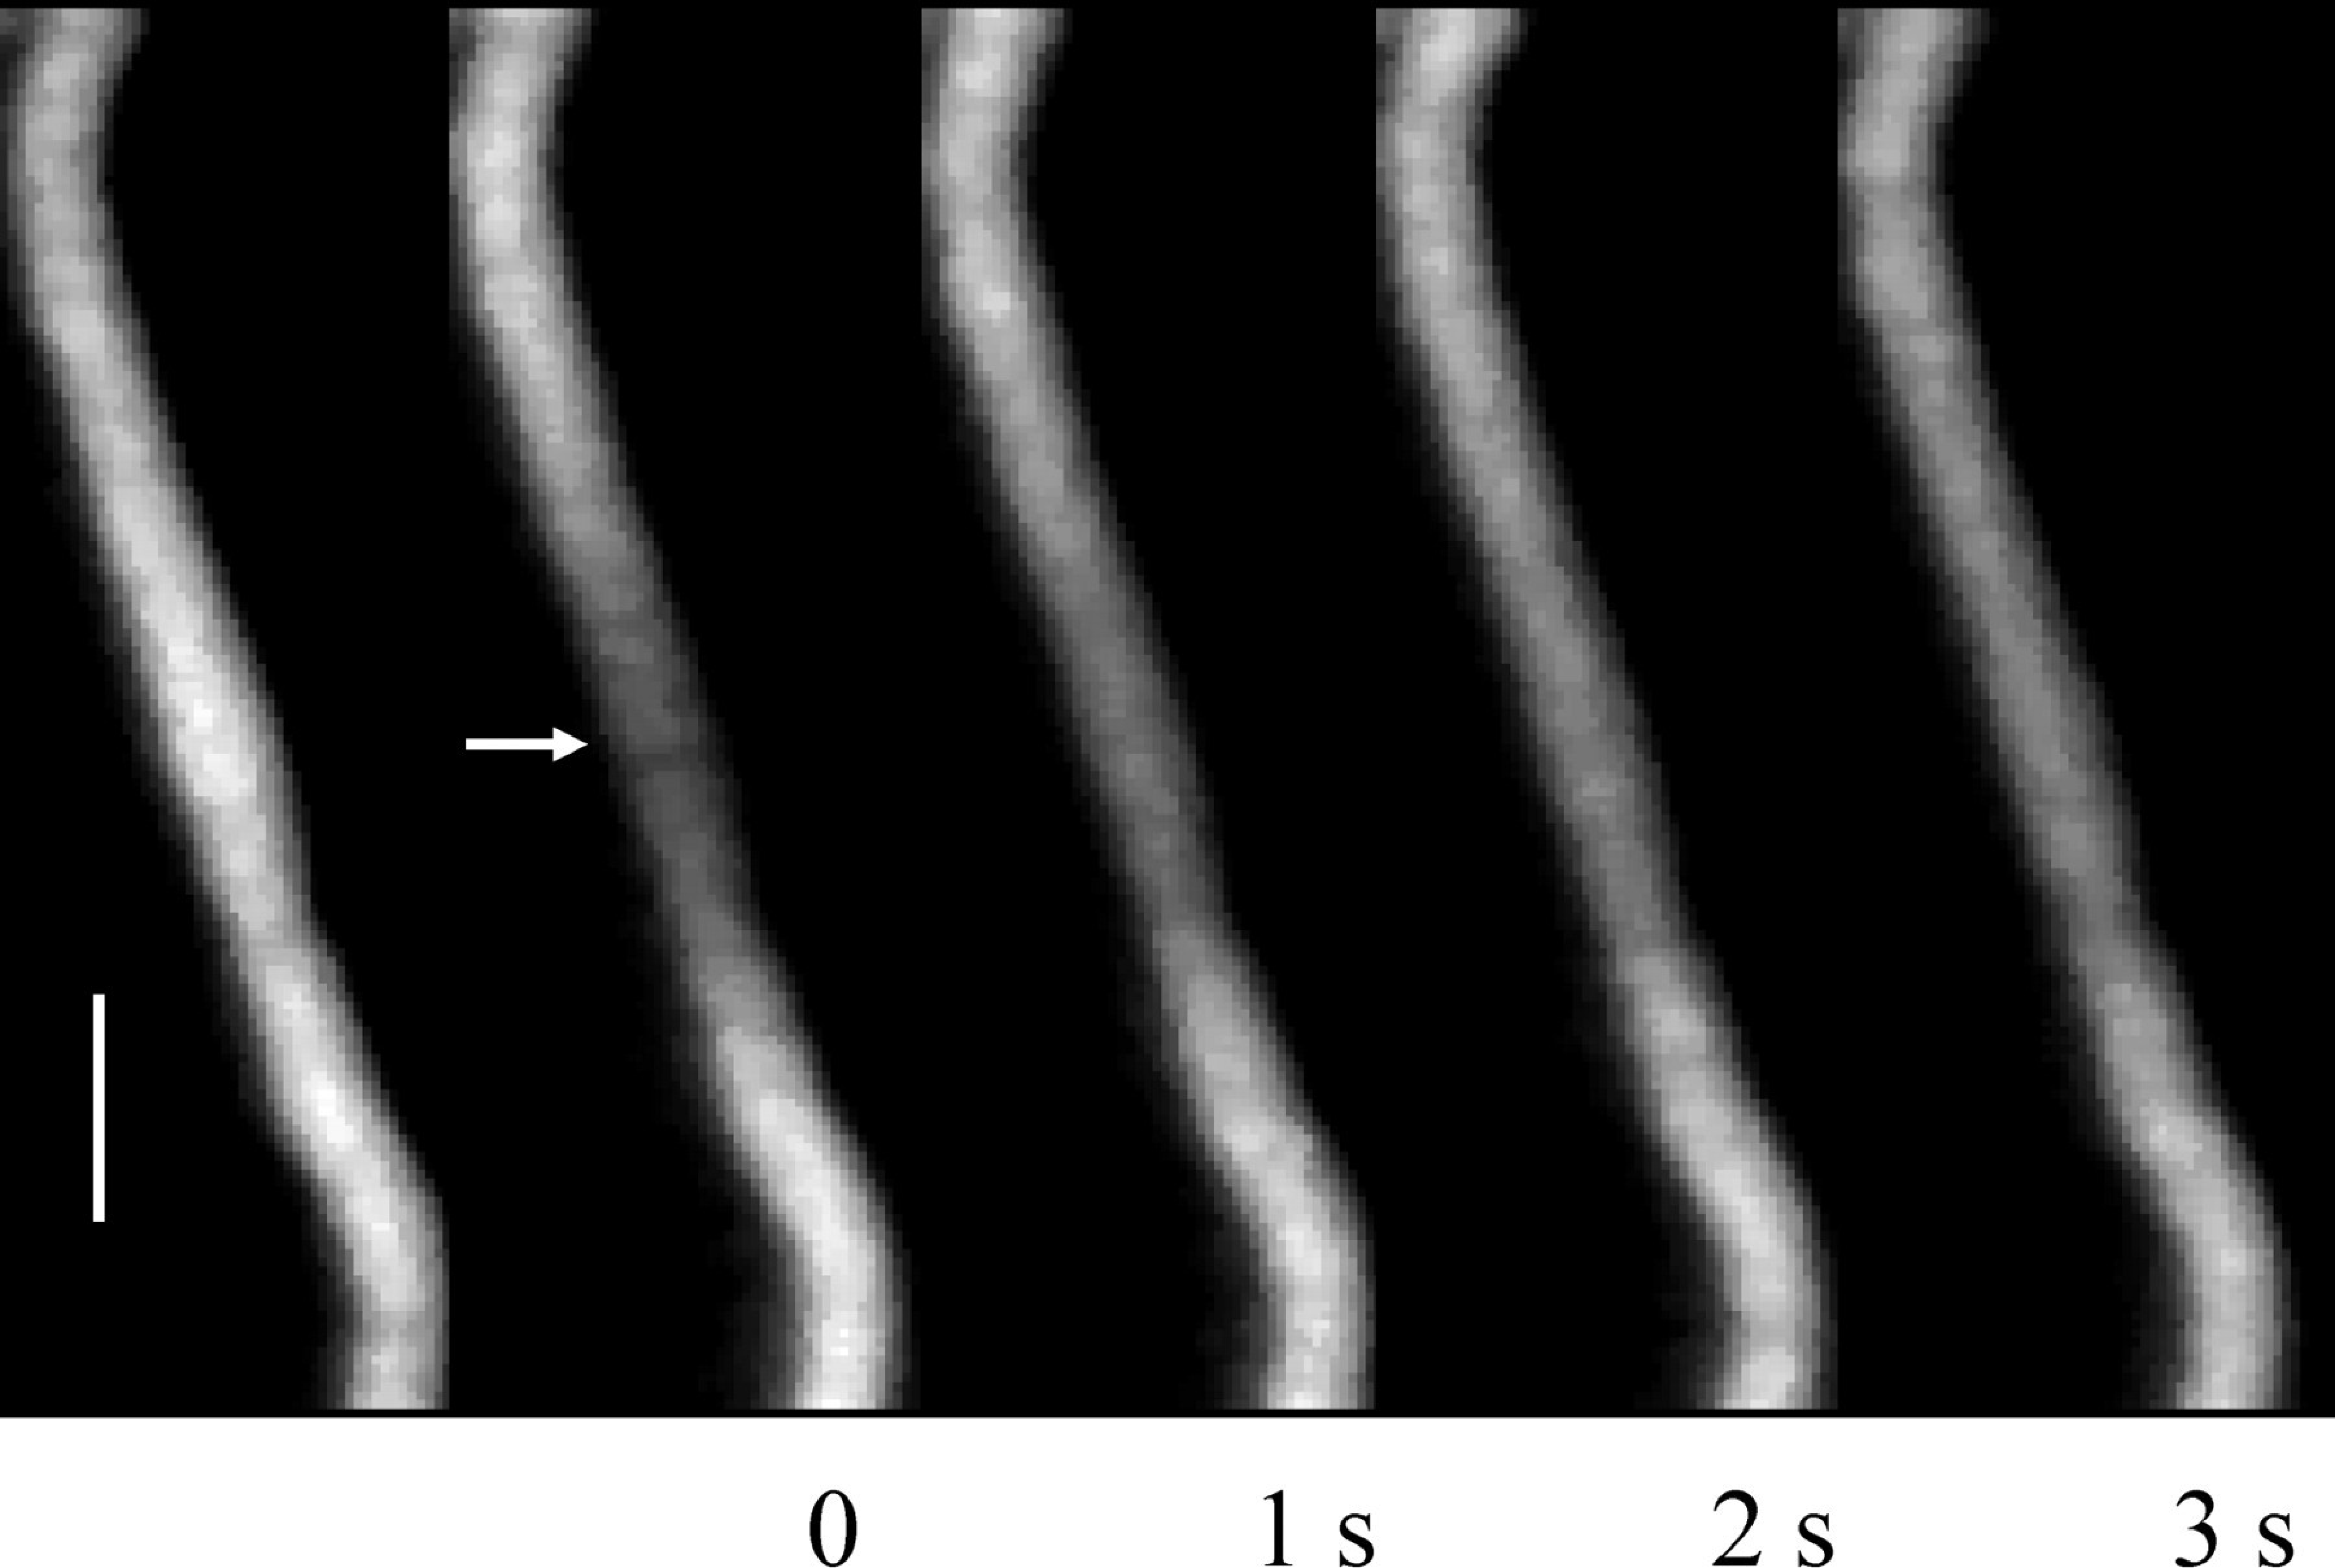
\includegraphics[height=50mm]{F5_large.pdf}

As fluorescent proteins from \textit{outside} that area diffuse
in (frames 1s to 3s), the bleached area becomes more fluorescent. By
measuring the rate at which the fluorescence returns, you can find out
how quickly the proteins are diffusing within the cell. The image
below shows the difference in fluorescence immediately after bleaching
(dark jagged line) and 4 seconds after (light jagged line), along with
fits to the data (smooth lines).

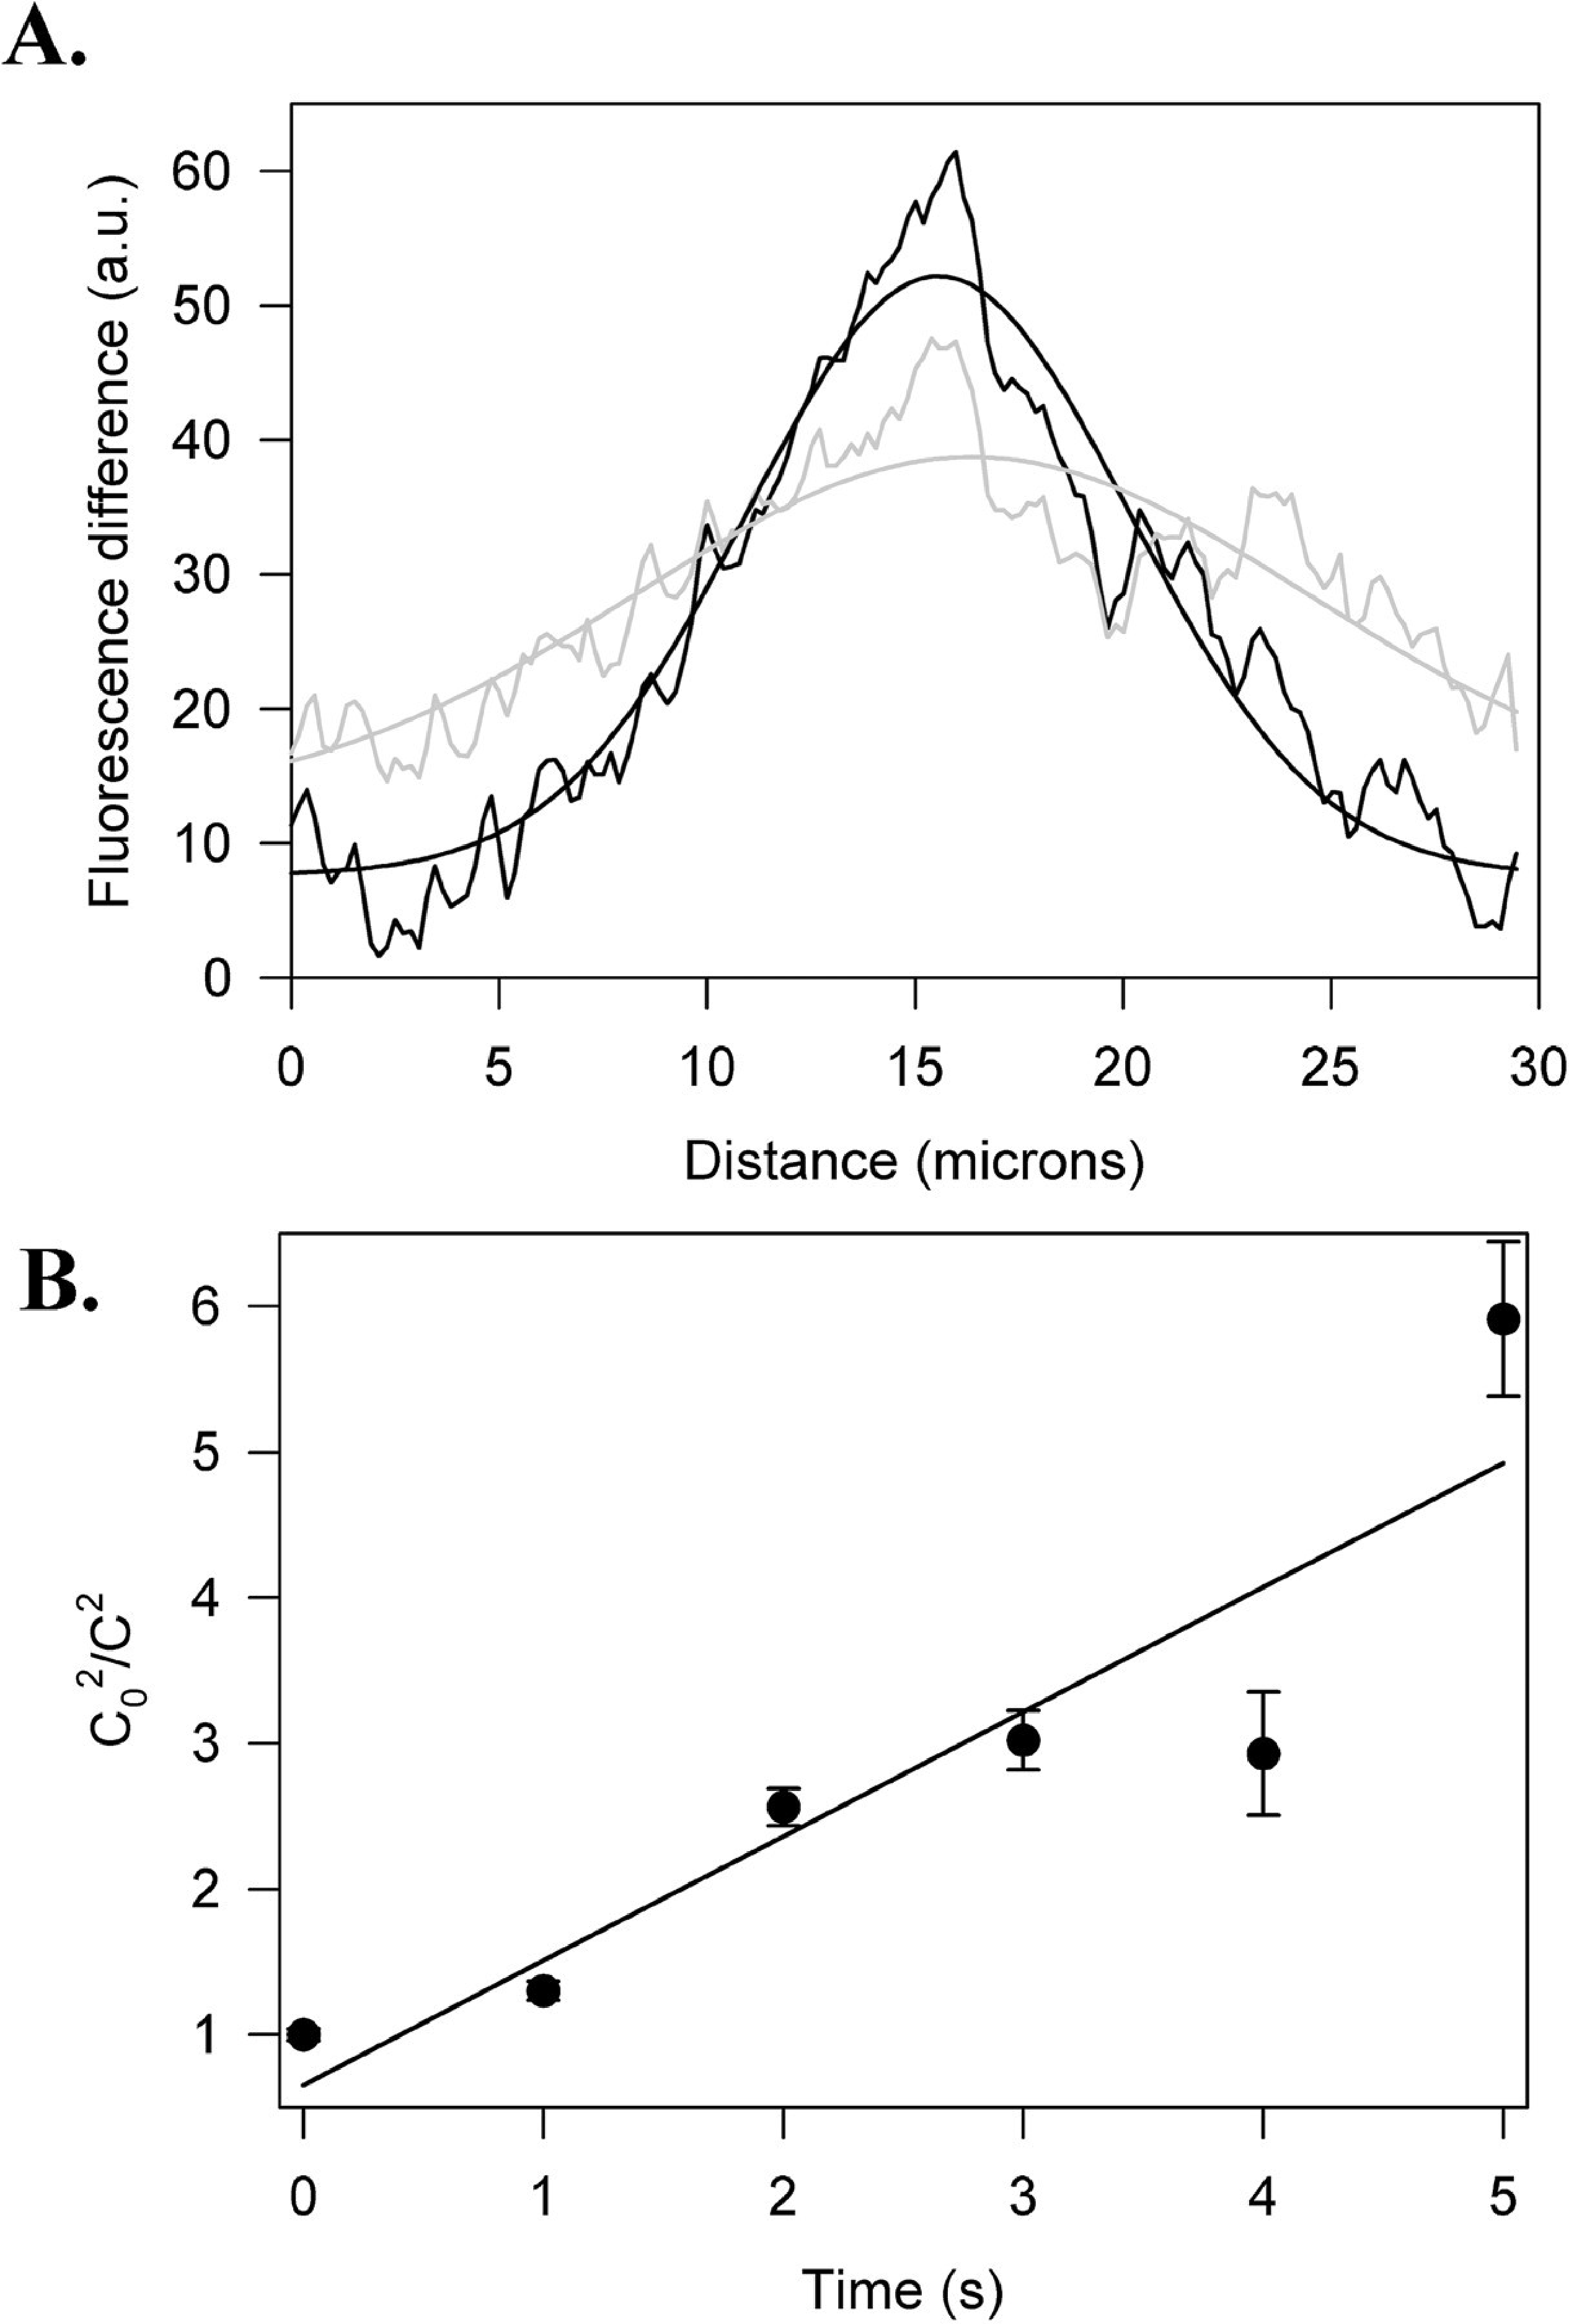
\includegraphics[trim = 10mm 300mm 00mm 30mm, clip, height=50mm]{F6_large.pdf}

Your goal is to write down an equation modeling the concentration of
protein over time. We'll split this problem up into three weeks. 

\subsection{Last week}
What PDE will you use to model the system? What are your initial
conditions? What are your boundary conditions? Will you be expanding
your solution in terms of $\sin$ or $\cos$ functions?

You should have decided to use the diffusion equation

\begin{equation}
  \label{eq:diff}
  \pd{c}{t} = D\pdd{c}{x}
\end{equation}
where $D$ is the diffusion constant and $c(x,t)$ is the concentration
of fluorescent molecules. There are a couple of ways you could have
modeled the initial conditions, depending on how you chose boundary
conditions. The simplest thing to do is to decide that you're
photobleaching a region from $-a$ to $a$, and that you have an
infinite amount of fluorophores. In that case, you'd get

\begin{equation*}
c(x,0) = \left\{\begin{matrix}
 c_0 & x < -a\\ 
 0 &-a < x < a\\ 
 c_0  &x < a
\end{matrix}\right.
\end{equation*}
but let's be a little more realistic. Let's assume we have a cell of
length $2L$, starting with a uniform concentration of $c_0$, and that
we bleach that same region. In this case, we get two restrictions. The
first tells us about the concentration:

\begin{equation}
\label{eq:cond1}
c(x,0) = \left\{\begin{matrix}
 c_0 &-L < x < -a\\ 
 0 &-a < x < a\\ 
 c_0  &a < x < L 
\end{matrix}\right.
\end{equation}
the second tells us that nothing flows into or out of the cell. If you
recall our class discussion, we write that as

\begin{equation}
\label{eq:cond2}
  \pd{c(x,t)}{x} = 0 \text{ for }x=\pm L
\end{equation}
and, given those boundary conditions, we can guess that we'll expand
our solution in cosines:


\begin{equation}
  \label{eq:solform}
  c(x,t) = A_0(t) + \sum_{n=1}^\infty A_n(t)\cos\left(\frac{x}{L}n\pi\right)
\end{equation}

\subsection{This week}
Your goal this week is to solve \eqref{eq:diff} subject to
\eqref{eq:cond1} and \eqref{eq:cond2}. I'll sketch the solution and
you can fill in the pieces. Alternatively, you can solve it however
you'd like!



\subsubsection{}
First, we plug \eqref{eq:solform} into \eqref{eq:diff}, yielding
\begin{equation}
  \pd{A_0}{t} + \sum_{n=1}^{\infty}(??) = D\sum(??)
\end{equation}

\answer{
Just plugging in directly leads to
\[
  \pd{A_0}{t} + \sum_{n=1}^{\infty}
\pd{A_n(t)}{t}
\cos\left(\frac{x}{L}n\pi\right)
 = D\sum_{n=1}^{\infty}
\left(-A_n(t)\frac{n^2\pi^2}{L^2}
\right)
\cos\left(\frac{x}{L}n\pi\right)
\]
}
\subsubsection{}
which gives us an infinite number of differential equations ({\bf
  why??}) 

\answer{This is just reminding you that the sum splits into separate equations}

that look like


\begin{eqnarray}
  \pd{A_0}{t} &=& ??,\\
  \pd{A_n}{t} &=& ??\qquad (n\ge 1)
\end{eqnarray}

\answer{
\begin{eqnarray}
  \pd{A_0}{t} &=& 0,\\
  \pd{A_n}{t} &=& -\frac{Dn^2\pi^2}{L^2}A_n(t)\qquad (n\ge 1)
\end{eqnarray}
}

These have solution

\begin{equation}
  A_n(t) = A_n(0)\cdot(??)
\end{equation}

\answer{
\[
  A_n(t) = A_n(0)e^{-(Dn^2\pi^2/L^2)t}
\]
}

We can use those formulas for $A_0$ and $A_n$ to rewrite
\eqref{eq:solform} as

\begin{equation}
\label{eq:solform2}
  ??
\end{equation}
\answer{
\[
  c(x,t) = A_0(t) + \sum_{n=1}^\infty 
A_n(0)e^{-(Dn^2\pi^2/L^2)t}
\cos\left(\frac{x}{L}n\pi\right)
 \]
}

which is our series solution, and has everything we need except for
the actual values of the amplitudes $A_n(0)$.

In order to get the amplitudes, we need to use the orthogonality of
cosines again. We play the standard trick for these sorts of problems,
and multiply both sides of \eqref{eq:solform2} by $\cos(n\pi x/L)$ for
different values of $n$ and then integrate over $x$. What does ``the
orthogonality of cosines'' mean in this case?


\begin{equation}
  ??
\end{equation}

\answer{
\[
\int_{-L}^L
\cos\left(\frac{x}{L}n\pi\right)
\cos\left(\frac{x}{L}m\pi\right)
dx = L\delta_{n,m}
\]
}

specifically, which integrals will you calculate to find the
coefficients?

\begin{equation}
  ??
\end{equation}

\answer{
Multiply both sides by $\cos(n\pi x/L)$ and integrate against $x$
\begin{eqnarray}
A_0(0) &=& \frac{1}{2L} \int_{-L}^Lc(x,0)dx\\
A_n(0) &=& \frac{1}{L} \int_{-L}^Lc(x,0)\cos\left(\frac{x}{L}n\pi\right) dx \qquad (n\ge 1)
\end{eqnarray}

}

{\bf Fill in all of the ``??'' spots above.} Next time, we'll finish
the solution and plot the results!

After all of that, we can evaluate the above integrals to get

\notes{
\begin{eqnarray}
A_0(0) &=& c_0\frac{L-a}{L}\\
A_n(0) &=& -2c_0\frac{\sin(n\pi a/L)}{n\pi} \qquad (n\ge 1)
\end{eqnarray}
}

Put those back into our formula for $c(x,t)$, and we can plot the
result! Do it, setting $a=L/2$. What happens at long times? What do we
mean by ``long times''?

You might want to plot the ``FRAP recovery curve'' i.e. $N_f(t)$, the
number of molecules in the region at time $t$.
\end{document}
